\section{TÍCH VÔ HƯỚNG CỦA HAI VÉCTƠ}

\subsection{TÓM TẮT LÝ THUYẾT}
\subsubsection{Góc giữa hai véc tơ: }
\begin{enumerate}[\iconMT]
	\item \indam{Cách dựng:} \immini{Cho hai vectơ $\overrightarrow{a}$ và $\overrightarrow{b}$ đều khác vectơ $\overrightarrow{0}$. Từ một điểm $O$ bất kì ta vẽ $\overrightarrow{OA}=\overrightarrow{a}$ và $\overrightarrow{OB}=\overrightarrow{b}$. Góc $\widehat{AOB}$ với số đo từ $0^\circ$ đến $180^\circ$ được gọi là góc giữa hai vectơ $\overrightarrow{a}$ và $\overrightarrow{b}$. Ta kí hiệu góc giữa hai vectơ $\overrightarrow{a}$ và $\overrightarrow{b}$ là $(\overrightarrow{a},\overrightarrow{b} )$.
	}{\begin{tikzpicture}[scale=0.5,font=\footnotesize,line join=round,line cap=round,>=stealth]
			\tkzDefPoints{0/0/O,3/3/A,-2.5/1/B, 3/0/C, 7/0/D}
			\tkzDefPointBy[translation=from O to A](C) \tkzGetPoint{C'}
			\tkzDefPointBy[translation=from O to B](D) \tkzGetPoint{D'}
			\tkzDrawSegments[->](O,A O,B C,C' D,D')
			\tkzLabelPoints[above](A,B)
			\tkzLabelPoints[below](O)
			\tkzLabelSegment(C,C'){$ \overrightarrow{a} $}
			\tkzLabelSegment(D,D'){$ \overrightarrow{b} $}
			\tkzMarkAngles(A,O,B)
	\end{tikzpicture}}
	\item \indam{Lưu ý:}
	\begin{listEX}[2]
		\item [\ding{172}] $(\overrightarrow{a},\overrightarrow{b} )=(\overrightarrow{b},\overrightarrow{a} )$. 
		\item [\ding{173}] $\vec{a}$ cùng hướng $\vec{b}$ thì $(\overrightarrow{a},\overrightarrow{b} )=0^\circ$
		\item [\ding{174}] $\vec{a}$ ngược hướng $\vec{b}$ thì $(\overrightarrow{a},\overrightarrow{b} )=180^\circ$
		\item [\ding{175}] $\vec{a}$ vuông góc $\vec{b}$ thì $(\overrightarrow{a},\overrightarrow{b} )=90^\circ$
	\end{listEX}
\end{enumerate}

\subsubsection{Tích vô hướng của hai vectơ} 
\begin{itemize}
	\item [\iconMT] \indam{Định nghĩa:}Cho hai véc-tơ $\overrightarrow{a}$ và $\overrightarrow{b}$ đều khác véc-tơ $\overrightarrow{0}$ Tích vô hướng của $\overrightarrow{a}$ và $\overrightarrow{b}$ là một số, kí hiệu là $\overrightarrow{a}\cdot\overrightarrow{b}$, được xác định bởi công thức sau:
	\boxmini{$\overrightarrow{a}\cdot \overrightarrow{b}=\left|\overrightarrow{a}\right|\cdot \left|\overrightarrow{b}\right|\cos\left(\overrightarrow{a},\overrightarrow{b}\right)$}
	\begin{luuy}
		Trường hợp ít nhất một trong hai véc-tơ $\overrightarrow{a}$ và $\overrightarrow{b}$ bằng véc-tơ $\vec{0}$ ta quy ước $\overrightarrow{a}\cdot\overrightarrow{b}=0$.
	\end{luuy}
	\item [\iconMT] \indam{Lưu ý:}
		\begin{itemize}
			\item Với $\overrightarrow{a}$ và $\overrightarrow{b}$ khác véc-tơ $\overrightarrow{0}$ ta có $\overrightarrow{a}\cdot\overrightarrow{b}=0\Leftrightarrow \overrightarrow{a}\perp \overrightarrow{b}$. 
			\item Khi $\overrightarrow{a}=\overrightarrow{b}$ tích vô hướng $\overrightarrow{a}\cdot\overrightarrow{a}$ được kí hiệu là $\overrightarrow{a^2}$ và số này được gọi là bình phương vô hướng của véc-tơ $\overrightarrow{a}$. Ta có:
			\boxmini{$\overrightarrow{a}^2=|\overrightarrow{a}|\cdot|\overrightarrow{a}|\cdot \cos0^\circ=|\overrightarrow{a}|^2$}
		\end{itemize}
	\item [\iconMT] \indam{Tính chất:}
Với ba véc-tơ $\overrightarrow{a}$, $\overrightarrow{b}$, $\overrightarrow{c}$ bất kì và mọi số $k$ ta có:
\begin{tcolorbox}[colframe=orange,colback=white,boxrule=0.2mm]
		\begin{itemize}
			\item $\overrightarrow{a}\cdot \overrightarrow{b}=\overrightarrow{b}\cdot \overrightarrow{a}$ (tính chất giao hoán);
			\item $\overrightarrow{a}\left(\overrightarrow{b}+\overrightarrow{c}\right)=\overrightarrow{a}\cdot \overrightarrow{b}+\overrightarrow{a}\cdot \overrightarrow{c}$ (tính chất phân phối);
			\item $(k\overrightarrow{a})\cdot \overrightarrow{b}=k(\overrightarrow{a}\cdot \overrightarrow{b})=\overrightarrow{a}\cdot (k\overrightarrow{b})$;
			\item $\overrightarrow{a}^2\ge 0$;\quad $\overrightarrow{a}^2=0\Leftrightarrow \overrightarrow{a}=0$.
		\end{itemize}
\end{tcolorbox}
\end{itemize}
\subsubsection{Biểu thức tọa độ của tích vô hướng:}
Cho hai véc-tơ $\overrightarrow{a}=(a_1;a_2 )$ và $\overrightarrow{b}=(b_1;b_2 )$. 
\begin{itemize}
	\item [\iconMT] \indam{Biểu thức tọa độ:} $\overrightarrow{a}\cdot \overrightarrow{b}=a_1b_1+a_2b_2$.
	\item [\iconMT] \indam{Ứng dụng:}
	\begin{listEX}[1]
		\item [\ding{172}] Chứng minh vuông góc: \boxmini{$\overrightarrow{a}\perp \overrightarrow{b} \Leftrightarrow \overrightarrow{a} \cdot \overrightarrow{b}=0 \Leftrightarrow a_1b_1+a_2b_2=0$}
		\item [\ding{173}] Độ dài của véc-tơ \boxmini{$|\overrightarrow{a}|=\sqrt{a_1^2+a_2^2}$}
		\item [\ding{174}] Góc giữa hai véc-tơ: \boxmini{$\cos\left(\overrightarrow{a},\overrightarrow{b}\right)=\dfrac{\overrightarrow{a}\overrightarrow{b}}{|\overrightarrow{a}|\cdot\left|\overrightarrow{b}\right|}=\dfrac{a_1b_1+a_2b_2}{\sqrt{a_1^2+a_2^2}\cdot \sqrt{b_1^2+b_2^2}}$}
	\end{listEX}
\end{itemize}

\subsection{RÈN LUYỆN KĨ NĂNG GIẢI TOÁN}

\begin{dang}{Tính tích vô hướng bằng định nghĩa}
	\begin{listEX}[1]
		\item [\ding{172}] Tính tích vô hướng: $\overrightarrow{AB} \cdot \overrightarrow{AC} = AB \cdot AC \cdot \cos A$.
		\item [\ding{173}] Tính độ dài: $\overrightarrow{AB}^2=AB^2$.
		\item [\ding{174}] Chứng minh vuông góc: $AB$ vuông góc với $CD$ khi $\overrightarrow{AB} \cdot \overrightarrow{CD}=0$. 
	\end{listEX}
\end{dang}

\begin{vd}%[Phan Văn Thành, dự án 10-DCHT-L1]%[0H2B2-1]
	Cho $\triangle ABC$ vuông tại $A$ có $AB = a$, $BC = 2a$. Tính các tích vô hướng
	\begin{tasks}(3)
		\task $\overrightarrow{AB}\cdot \overrightarrow{AC}$.
		\task $\overrightarrow{AC} \cdot \overrightarrow{CB}$.
		\task $\overrightarrow{AB}\cdot \overrightarrow{BC}$.
	\end{tasks}
\loigiai{
\begin{enumerate}[a)]
	\item Do $\triangle ABC$ vuông tại $A$ nên $\overrightarrow{AB}\cdot \overrightarrow{AC} = 0$.
	\item Do $\triangle ABC$ vuông tại $A$ nên $AC^2 = BC^2 - AB^2 = 3a^2 \Rightarrow AC = a\sqrt{3}$.\\
	Khi đó $\overrightarrow{AC} \cdot \overrightarrow{CB} = \left|\overrightarrow{AC}\right| \cdot \left|\overrightarrow{CB}\right|\cdot \cos \left(\overrightarrow{AC}, \overrightarrow{CB}\right) = - AC \cdot BC \cdot \cos C = - a\sqrt{3} \cdot 2a \cdot \dfrac{a\sqrt{3}}{2a} = -3a^2$.
	\item Ta có $\overrightarrow{AB}\cdot \overrightarrow{BC} = \left|\overrightarrow{AB}\right| \cdot \left|\overrightarrow{BC}\right|\cdot \cos \left(\overrightarrow{AB}, \overrightarrow{BC}\right) = - AB \cdot BC \cdot \cos B = - a \cdot 2a \cdot \dfrac{a}{2a} = -a^2$.
\end{enumerate}
}
\end{vd}\dongcham{5}

\begin{vd}%[Phan Văn Thành, dự án 10-DCHT-L1]%[0H2K2-1]
	Cho $\triangle ABC$ đều cạnh bằng $a$. Tính các tích vô hướng
	\begin{tasks}(3)
		\task $\overrightarrow{AB}\cdot \overrightarrow{AC}$.
		\task $\overrightarrow{AC} \cdot \overrightarrow{CB}$.
		\task $\overrightarrow{AB}\cdot \overrightarrow{BC}$.
	\end{tasks}
	\loigiai{
		\begin{enumerate}[a)]
			\item Ta có $\overrightarrow{AB}\cdot \overrightarrow{AC} = \left|\overrightarrow{AB}\right| \cdot \left|\overrightarrow{AC}\right|\cdot \cos \left(\overrightarrow{AB}, \overrightarrow{AC}\right) = AB \cdot AC \cdot \cos A = a \cdot a \cdot \cos 60^\circ =\dfrac{1}{2}a^2$.
			\item Ta có $\overrightarrow{AC}\cdot \overrightarrow{CB} = \left|\overrightarrow{AC}\right| \cdot \left|\overrightarrow{CB}\right|\cdot \cos \left(\overrightarrow{AC}, \overrightarrow{CB}\right) = AC \cdot CB \cdot \cos C = - a \cdot a \cdot \cos 60^\circ = -\dfrac{1}{2}a^2$.
			\item Ta có $\overrightarrow{AB}\cdot \overrightarrow{BC} = \left|\overrightarrow{AB}\right| \cdot \left|\overrightarrow{BC}\right|\cdot \cos \left(\overrightarrow{AB}, \overrightarrow{BC}\right) = - AB \cdot BC \cdot \cos B = - a \cdot a \cdot \cos 60^\circ = -\dfrac{1}{2}a^2$.
	\end{enumerate}}
\end{vd}\dongcham{5}

\begin{vd}
	Cho hình vuông $ABCD$ tâm $O$, cạnh $a$. Tính giá trị của biểu thức sau
	\begin{tasks}(3)
		\task $\overrightarrow{AB}\cdot \overrightarrow{AC}$.
		\task $\overrightarrow{AC}\left(\overrightarrow{AB} + \overrightarrow{AD}\right)$.
		\task $\overrightarrow{OD}\cdot \overrightarrow{BC}$.
	\end{tasks}
	\loigiai{
		\begin{enumerate}[a)]
			\item $\overrightarrow{AB}\cdot \overrightarrow{AC} = AB \cdot AC \cdot \cos \widehat{BAC} = a \cdot a \cdot \cos 45^\circ = \dfrac{a^2\sqrt{2}}{2}$.
			\item $\overrightarrow{AC}\left(\overrightarrow{AB} + \overrightarrow{AD}\right) = \overrightarrow{AC} \cdot \overrightarrow{AC} = AC^2 = (a\sqrt{2})^2 = 2a^2$.
			\item Vì $ABCD$ là hình vuông nên $\overrightarrow{BC} = \overrightarrow{AD}$ và $\widehat{ADO} = 45^\circ$.
			Khi đó:
			\[ \overrightarrow{OD} \cdot \overrightarrow{BC} = \overrightarrow{OD} \cdot \overrightarrow{AD} = \left(-\overrightarrow{DO}\right) \cdot \left(-\overrightarrow{DA}\right) = \overrightarrow{DO} \cdot \overrightarrow{DA}. \]
			Góc giữa hai véc-tơ $\overrightarrow{DO}$ và $\overrightarrow{DA}$ chính là góc $\widehat{ADO} = 45^\circ$. Độ dài $DO = \dfrac{1}{2}BD = \dfrac{a\sqrt{2}}{2}$.
			\[ \overrightarrow{DO} \cdot \overrightarrow{DA} = \left|\overrightarrow{DO}\right| \cdot \left|\overrightarrow{DA}\right| \cdot \cos 45^\circ = \dfrac{a\sqrt{2}}{2} \cdot a \cdot \dfrac{\sqrt{2}}{2} = \dfrac{a^2}{2}. \]
			Vậy $\overrightarrow{OD} \cdot \overrightarrow{BC} = \dfrac{a^2}{2}$.
	\end{enumerate}}
\end{vd}\dongcham{8}

\begin{vd}
	\immini{
		Cho hình vuông $ABCD$. Gọi $M$ và $N$ lần lượt là trung điểm của các cạnh $BC$ và $CD$. Chứng minh rằng hai đường thẳng $AM$ và $BN$ vuông góc với nhau.
	}{
		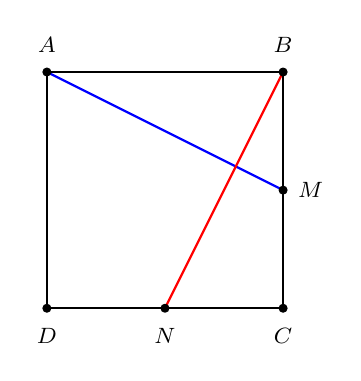
\begin{tikzpicture}[scale=1, font=\footnotesize, line join=round, line cap=round, >=stealth]
			\def\a{3} % Độ dài cạnh hình vuông
			\coordinate (A) at (0,\a);
			\coordinate (B) at (\a,\a);
			\coordinate (C) at (\a,0);
			\coordinate (D) at (0,0);
			\coordinate (M) at (\a,\a/2);
			\coordinate (N) at (\a/2,0);
			
			\draw[thick] (A)--(B)--(C)--(D)--cycle;
			\draw[blue, thick] (A)--(M);
			\draw[red, thick] (B)--(N);
			
			\foreach \x/\g in {A/90,B/90,C/-90,D/-90,M/0,N/-90}\draw[fill=black] (\x) circle (.05) +(\g:.35)node{\footnotesize$\x$};
		\end{tikzpicture}
	}
	\loigiai{
		\immini{	Đặt cạnh của hình vuông $ABCD$ là $a$. Ta sử dụng phương pháp véc-tơ để chứng minh.\\
			Ta có:
			\begin{itemize}
				\item $\overrightarrow{AM} = \overrightarrow{AB} + \overrightarrow{BM} = \overrightarrow{AB} + \dfrac{1}{2}\overrightarrow{BC}$.
				\item $\overrightarrow{BN} = \overrightarrow{BC} + \overrightarrow{CN} = \overrightarrow{BC} + \dfrac{1}{2}\overrightarrow{CD} = \overrightarrow{BC} - \dfrac{1}{2}\overrightarrow{AB}$ (vì $\overrightarrow{CD} = -\overrightarrow{AB}$).
			\end{itemize}
		}{
		}
		Xét tích vô hướng của hai véc-tơ $\overrightarrow{AM}$ và $\overrightarrow{BN}$:
		\begin{align*}
			\overrightarrow{AM} \cdot \overrightarrow{BN} &= \left( \overrightarrow{AB} + \dfrac{1}{2}\overrightarrow{BC} \right) \cdot \left( \overrightarrow{BC} - \dfrac{1}{2}\overrightarrow{AB} \right) \\
			&= \overrightarrow{AB} \cdot \overrightarrow{BC} - \dfrac{1}{2}\overrightarrow{AB}^2 + \dfrac{1}{2}\overrightarrow{BC}^2 - \dfrac{1}{4}\overrightarrow{BC} \cdot \overrightarrow{AB}
		\end{align*}
		Vì $ABCD$ là hình vuông nên $AB \perp BC \Rightarrow \overrightarrow{AB} \cdot \overrightarrow{BC} = 0$. \\
		Đồng thời $|\overrightarrow{AB}| = |\overrightarrow{BC}| = a$, nên $\overrightarrow{AB}^2 = a^2$ và $\overrightarrow{BC}^2 = a^2$.\\
		Thay vào biểu thức trên ta được:
		\[ \overrightarrow{AM} \cdot \overrightarrow{BN} = 0 - \dfrac{1}{2}a^2 + \dfrac{1}{2}a^2 - 0 = 0. \]
		Vì $\overrightarrow{AM} \cdot \overrightarrow{BN} = 0$ nên $AM \perp BN$. (đpcm)
	}
\end{vd}
\dongcham{5}
\begin{vd}
	\immini{
		Trong dự án cải tạo cảnh quan của trường, tổ Toán hợp tác cùng học sinh thiết kế một khung mái che có dạng tam giác cân $ABC$ với $AB = AC$. Để đảm bảo tính chịu lực và tính thẩm mỹ, một thanh chống thẳng đứng được lắp đặt nối từ đỉnh $A$ xuống trung điểm $M$ của thanh xà ngang $BC$. Bằng kiến thức véc-tơ, hãy chứng minh rằng thanh chống $AM$ luôn vuông góc với thanh xà ngang $BC$.
	}{
		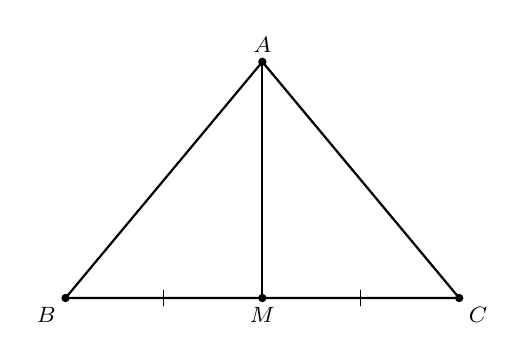
\begin{tikzpicture}[>=stealth, scale=1, font=\footnotesize, line join=round, line cap=round]
			\coordinate (M) at (0,0);
			\coordinate (B) at (-2.5,0);
			\coordinate (C) at (2.5,0);
			\coordinate (A) at (0,3);
			
			\draw[thick] (A) -- (B) -- (C) -- cycle;
			\draw[thick] (A) -- (M);
			
			\fill (A) circle (1.5pt) node[above] {$A$};
			\fill (B) circle (1.5pt) node[below left] {$B$};
			\fill (C) circle (1.5pt) node[below right] {$C$};
			\fill (M) circle (1.5pt) node[below] {$M$};
					% Ký hiệu bằng nhau
			\draw (-1.25,-0.1) -- (-1.25,0.1);
			\draw (1.25,-0.1) -- (1.25,0.1);
		\end{tikzpicture}
	}
	\loigiai{
		Ta cần chứng minh $\vec{AM} \cdot \vec{BC} = 0$.
		Vì $M$ là trung điểm của $BC$ nên ta có:
		$$\vec{AM} = \dfrac{1}{2}(\vec{AB} + \vec{AC})$$
		Véc-tơ cạnh đáy được biểu diễn là: 
		$$\vec{BC} = \vec{AC} - \vec{AB}$$
		Xét tích vô hướng:
		$$\vec{AM} \cdot \vec{BC} = \dfrac{1}{2}(\vec{AB} + \vec{AC}) \cdot (\vec{AC} - \vec{AB}) = \dfrac{1}{2}(\vec{AC}^2 - \vec{AB}^2)$$
		Do tam giác $ABC$ cân tại $A$ nên $AC = AB$, suy ra $AC^2 - AB^2 = 0$.
		Vậy $\vec{AM} \cdot \vec{BC} = 0$, kết luận thanh chống $AM$ hoàn toàn vuông góc với thanh xà $BC$.
	}
\end{vd}
\dongcham{5}
\begin{dang}{Biểu thức tọa độ của tích vô hướng}
	Cho véc-tơ $\overrightarrow{a}=(a_1;a_2 )$, $\overrightarrow{b}=(b_1;b_2 )$. Khi đó, ta có các công thức sau:
	\begin{listEX}[1]
		\item [\ding{172}] Tính tích vô hướng: $\boxed{\overrightarrow{a}\cdot \overrightarrow{b}=a_1b_1+a_2b_2}$
		\item [\ding{173}] Tính độ dài: $\boxed{|\overrightarrow{a}|=\sqrt{a_1^2+a_2^2}}$.
		\item [\ding{174}] Tính góc: $\boxed{\cos\left(\overrightarrow{a},\overrightarrow{b}\right)=\dfrac{\overrightarrow{a}\overrightarrow{b}}{|\overrightarrow{a}|\cdot\left|\overrightarrow{b}\right|}=\dfrac{a_1b_1+a_2b_2}{\sqrt{a_1^2+a_2^2}\cdot \sqrt{b_1^2+b_2^2}}}$
		\item [\ding{175}] Chứng minh vuông góc: \fbox{$\overrightarrow{a}\perp \overrightarrow{b} \Leftrightarrow a_1b_1+a_2b_2=0$}. 
	\end{listEX}
\end{dang}

\begin{vd}
	Trong mặt phẳng tọa độ $Oxy$, cho hai véc-tơ $\overrightarrow{a}=(1;-2)$, $\overrightarrow{b}=(2;4)$ và $\overrightarrow{c}=(3;-1)$.
	\begin{listEX}[2]
		\item Tính $\big|\overrightarrow{a}\big|$, $\big|\overrightarrow{b}\big|$
		\item Tính $\overrightarrow{a} \cdot \overrightarrow{b}$
		\item Tính $\overrightarrow{a} \cdot (\overrightarrow{b}+\overrightarrow{c})$
		\item Tính $\cos\left( \overrightarrow{a},\overrightarrow{b}\right)$
	\end{listEX}
	\loigiai{
		\begin{enumerate}[a)]
			\item Độ dài của các véc-tơ $\vec{a}$ và $\vec{b}$ là:
			\begin{itemize}
				\item $|\vec{a}| = \sqrt{1^2 + (-2)^2} = \sqrt{1 + 4} = \sqrt{5}$.
				\item $|\vec{b}| = \sqrt{2^2 + 4^2} = \sqrt{4 + 16} = \sqrt{20} = 2\sqrt{5}$.
			\end{itemize}
			\item Tích vô hướng của $\vec{a}$ và $\vec{b}$ là:
			\[ \vec{a} \cdot \vec{b} = 1 \cdot 2 + (-2) \cdot 4 = 2 - 8 = -6. \]
			\item Tọa độ của véc-tơ $\vec{b} + \vec{c}$ là:
			\[ \vec{b} + \vec{c} = (2 + 3; 4 + (-1)) = (5; 3). \]
			Khi đó, tích vô hướng cần tìm là:
			\[ \vec{a} \cdot (\vec{b} + \vec{c}) = 1 \cdot 5 + (-2) \cdot 3 = 5 - 6 = -1. \]
			\item Cô-sin của góc giữa hai véc-tơ $\vec{a}$ và $\vec{b}$ là:
			\[ \cos(\vec{a}, \vec{b}) = \dfrac{\vec{a} \cdot \vec{b}}{|\vec{a}| \cdot |\vec{b}|} = \dfrac{-6}{\sqrt{5} \cdot 2\sqrt{5}} = \dfrac{-6}{10} = -\dfrac{3}{5}. \]
		\end{enumerate}
}
\end{vd}\dongcham{8}

\begin{vd}%[Đỗ Duy An, dự án 10-DCHT-L1]%[0H2B2-3] 
	Trong mặt phẳng $Oxy$, cho ba véc-tơ $\overrightarrow{a}=(1;3)$, $\overrightarrow{b}=(6;-2)$, $\overrightarrow{c}=(x;1)$.
	\begin{tasks}(1)
		\task Chứng minh $\overrightarrow{a}\perp \overrightarrow{b}$.
		\task Tìm tất cả các giá trị của $x$ để $\overrightarrow{a}\perp \overrightarrow{c}$.
		\task Tìm tất cả các giá trị của $x$ để $\overrightarrow{a}$ cùng phương với $\overrightarrow{c}$.
		\task Tìm tọa độ véc-tơ $\overrightarrow{d}$ thỏa mãn $\overrightarrow{a}\perp \overrightarrow{d}$ và $\overrightarrow{b}\cdot\overrightarrow{d}=20$.
	\end{tasks}
	\loigiai{
		\begin{enumerate}[a)]
			\item Ta có $\overrightarrow{a}\cdot\overrightarrow{b}=1\cdot6-3\cdot2=0$ nên $\overrightarrow{a}
			\perp \overrightarrow{b}$.
			\item Ta có $\overrightarrow{a}\perp \overrightarrow{c}\Leftrightarrow x+3=0 \Leftrightarrow x=-3$.
			\item $\overrightarrow{a}$ cùng phương với $\overrightarrow{c}$ khi và chỉ khi $\overrightarrow{c}=k\overrightarrow{a}\Leftrightarrow (x;1)=k(1;3) \Leftrightarrow \heva{&x=k\\&1=3k}\Leftrightarrow \heva{&x=\dfrac{1}{3}\\&k=\dfrac{1}{3}.}$
			\item  Ta gọi tọa độ véc-tơ $\overrightarrow{d}=(x;y)$.\\
			Ta có $\heva{&\overrightarrow{a}\perp \overrightarrow{d}\\&\overrightarrow{b}\cdot\overrightarrow{d}=20} \Leftrightarrow \heva{&x+3y=0\\&6x-2y=20} \Leftrightarrow \heva{&x=3\\&y=-1}$. Vậy $\overrightarrow{d}=(3;-1)$.
	\end{enumerate}}
\end{vd}\dongcham{8}
\begin{dang}{Tọa độ điểm}
	\begin{itemize}
		\item [\ding{172}] Tọa độ véc tơ \fbox{$\overrightarrow{AB}=(x_B-x_A;y_B-y_A)$}.
		\item [\ding{173}] Độ dài đoạn thẳng $\boxed{AB=\sqrt{(x_B-x_A)^2+(y_B-y_A)^2}}$.
	\end{itemize}
\end{dang}

\begin{vd}
	Cho điểm $A(1;3)$ và $B(3;-1)$. Tính góc giữa hai véc tơ $\vec{OA}$ và $\vec{AB}$.
\loigiai{
	Ta có tọa độ các véc-tơ:
	\begin{itemize}
		\item $\overrightarrow{OA} = (1; 3)$.
		\item $\overrightarrow{AB} = (x_B - x_A; y_B - y_A) = (3 - 1; -1 - 3) = (2; -4)$.
	\end{itemize}
	Tích vô hướng của $\overrightarrow{OA}$ và $\overrightarrow{AB}$ là:
	\[ \overrightarrow{OA} \cdot \overrightarrow{AB} = 1 \cdot 2 + 3 \cdot (-4) = 2 - 12 = -10. \]
	Độ dài của các véc-tơ là:
	\begin{itemize}
		\item $\left|\overrightarrow{OA}\right| = \sqrt{1^2 + 3^2} = \sqrt{10}$.
		\item $\left|\overrightarrow{AB}\right| = \sqrt{2^2 + (-4)^2} = \sqrt{4 + 16} = \sqrt{20} = 2\sqrt{5}$.
	\end{itemize}
	Gọi $\alpha$ là góc giữa hai véc-tơ $\overrightarrow{OA}$ và $\overrightarrow{AB}$. Ta có:
	\[ \cos \alpha = \dfrac{\overrightarrow{OA} \cdot \overrightarrow{AB}}{\left|\overrightarrow{OA}\right| \cdot \left|\overrightarrow{AB}\right|} = \dfrac{-10}{\sqrt{10} \cdot 2\sqrt{5}} = \dfrac{-10}{2\sqrt{50}} = \dfrac{-10}{10\sqrt{2}} = -\dfrac{1}{\sqrt{2}} = -\dfrac{\sqrt{2}}{2}. \]
	Suy ra $\alpha = 135^\circ$.\\
	Vậy góc giữa hai véc-tơ $\overrightarrow{OA}$ và $\overrightarrow{AB}$ là $135^\circ$.
}
\end{vd}\dongcham{4}

\begin{vd}
	Cho tam giác $ABC$ có $A(1; 2)$, $B(-2; 6)$, $C(9; 8)$.
	\begin{tasks}(1)
		\task Tính $\overrightarrow{AB}\cdot \overrightarrow{AC}$. Chứng minh tam giác $ABC$ vuông tại $A$.
		\task Tìm tâm và bán kính đường tròn ngoại tiếp tam giác $ABC$.
		\task Tính chu vi, diện tích tam giác $ABC$.
		\task Tìm tọa độ điểm $N$ trên $Ox$ để tam giác $ANC$ cân tại $N$.
		\task Tìm tọa độ điểm $D$ để $ABDC$ là hình chữ nhật.
	\end{tasks}
	\loigiai{
		\begin{enumerate}
			\item Ta có $\overrightarrow{AB} = (-3; 4)$ và $\overrightarrow{AC} = (8; 6)$. Nên $\overrightarrow{AB} \cdot \overrightarrow{AC} = (-3)\cdot 8 + 4 \cdot 6 = 0$ nên $AB \perp AC$ hay $\triangle ABC$ vuông tại $A$.
			\item Do $\triangle ABC$ vuông tại $A$ nên tâm $I$ của đường tròn ngoại tiếp tam giác $ABC$ là trung điểm $BC$ và bán kính $R = \dfrac{BC}{2}$.\\
			Gọi $I(x; y)$ là trung điểm $BC$ nên $\heva{&x = \dfrac{-2 + 9}{2} = \dfrac{7}{2}\\&y = \dfrac{6 + 8}{2} = 7}$. Vậy $I\left(\dfrac{7}{2}; 7\right)$.\\
			Ta có $BC = \sqrt{(9 + 2)^2 + (8 - 6)^2} = 5\sqrt{5}$. Vậy $R = \dfrac{BC}{2} = \dfrac{5\sqrt{5}}{2}$.
			\item Ta có $AB = \sqrt{(-3)^2 + 4^2} = 5$, $AC = \sqrt{8^2 + 6^2} = 10$, $BC = 5\sqrt{5}$.\\
			Khi đó diện tích $\triangle ABC$ là $S_{\triangle ABC} = \dfrac{1}{2}AB \cdot AC = 25$ và chu vi $\triangle ABC$ là $P_{\triangle ABC} = 15 + 5\sqrt{5}$.
			\item Do $N \in Ox$ nên $N(x; 0)$. Ta có $NA = \sqrt{(x - 1)^2 + 4}$ và $NC = \sqrt{(x - 9)^2 + 64}$.\\
			Do $\triangle ANC$ cân tại $N$ nên $NA^2 = NC^2 \Leftrightarrow x^2 - 2x + 5 = x^2 - 18x + 145 \Leftrightarrow 16x = 140 \Leftrightarrow x = \dfrac{35}{4}$. Vậy $N\left(\dfrac{35}{4}; 0\right)$.
			\item Gọi $D(x; y)$ là điểm cần tìm. Ta có $\overrightarrow{AD} = (x - 1; y - 2)$ và $\overrightarrow{BC} = (11; 2)$.\\
			Do $\triangle ABC$ vuông tại $A$ nên $ABCD$ là hình chữ nhật $\Rightarrow \overrightarrow{AD} = \overrightarrow{BC} \Leftrightarrow \heva{&x - 1 =11\\&y - 2 = 2} \Leftrightarrow \heva{&x = 12\\&y = 4}$. Vậy $D(12; 4)$.
		\end{enumerate}
	}
\end{vd}\dongcham{21}

\begin{dang}{Xác định tọa độ các điểm đặc biệt trong tam giác}
		\begin{itemize}
		
			\item [\ding{172}] Xác định tọa độ trực tâm $H$ của tam giác $ABC$.
			\begin{gachsoc}
				\immini{\begin{itemize}
						\item [$\bullet$] Trực tâm $H$ là giao ba đường cao.
						\item [$\bullet$] Gọi $H(a;b)$ là trực tâm tam giác $ABC$.
						\item [$\bullet$] Giải hệ điều kiện $\heva{& \overrightarrow{AH} \cdot \overrightarrow{BC}=0\\& \overrightarrow{BH} \cdot \overrightarrow{AC}=0}$, tìm $a$, $b$.
					\end{itemize}
				}{
					\begin{tikzpicture}[scale=1, line join=round, line cap=round]
						\tkzDefPoints{0/0/B,3/0/C,1/2/A}
						\tkzDefPointBy[projection=onto C--B](A)\tkzGetPoint{K}
						\tkzDefPointBy[projection=onto A--B](C)\tkzGetPoint{E}
						\tkzDefPointBy[projection=onto C--A](B)\tkzGetPoint{F}
						\tkzInterLL(A,K)(C,E)\tkzGetPoint{H}	
						\pgfresetboundingbox
						\tkzDrawPolygon(A,B,C)
						\tkzDrawSegments(A,K C,E B,F)
						\tkzLabelPoints[below](B,C,K)
						\tkzLabelPoints[below right](H)
						\tkzLabelPoints[above](A)
						\tkzLabelPoints[right](F)
						\tkzLabelPoints[left](E)
				\end{tikzpicture}}
			\end{gachsoc}
			\item [\ding{173}] Xác định tọa độ hình chiếu vuông góc của $A$ lên $BC$
			\begin{gachsoc}
				\immini{\begin{itemize}
						\item [$\bullet$] Gọi $K(a;b)$ là hình chiếu vuông góc của $A$ lên $BC$.
						\item [$\bullet$] Giải hệ điều kiện $\heva{& \overrightarrow{AK} \cdot \overrightarrow{BC}=0\\& \overrightarrow{BK} \text{ cùng phương } \overrightarrow{BC}}$, tìm $a$, $b$.
					\end{itemize}
				}{
					\begin{tikzpicture}[scale=1, line join=round, line cap=round]
						\tkzDefPoints{0/0/B,3/0/C,1/2/A}
						\tkzDefPointBy[projection=onto C--B](A)\tkzGetPoint{K}
						\tkzDefPointBy[projection=onto A--B](C)\tkzGetPoint{E}
						\tkzDefPointBy[projection=onto C--A](B)\tkzGetPoint{F}
						\pgfresetboundingbox
						\tkzDrawPolygon(A,B,C)
						\tkzDrawSegments(A,K C,E B,F)
						\tkzLabelPoints[below](B,C,K)
						\tkzLabelPoints[above](A)
						\tkzLabelPoints[right](F)
						\tkzLabelPoints[left](E)
				\end{tikzpicture}}
			\end{gachsoc}
			\item [\ding{174}] Xác định tọa độ tâm đường tròn ngoại tiếp tam giác $ABC$.
			\begin{gachsoc}
				\immini{\begin{itemize}
						\item [$\bullet$] Tâm đường tròn ngoại tiếp là giao của ba đường trung trực.
						\item [$\bullet$] Gọi $I(a;b)$ là tâm đường tròn ngoại tiếp tam giác $ABC$.
						\item [$\bullet$] Giải hệ điều kiện $\heva{& IA =IB\\& IA=IC}$, tìm $a$, $b$.
					\end{itemize}
				}{
					\begin{tikzpicture}[scale=0.9, line join=round, line cap=round]
						\tkzDefPoints{0/0/B,3/0/C,1/2/A}
						\tkzCircumCenter(A,B,C)\tkzGetPoint{I}
						\tkzDrawCircle[circum](A,B,C)
						\tkzDrawSegments(I,A I,B I,C)
						\tkzDrawPolygon(A,B,C)
						\tkzLabelPoints[below,font=\footnotesize](I)
						\tkzLabelPoints[above,font=\footnotesize](A)
						\tkzLabelPoints[below left,font=\footnotesize](B)
						\tkzLabelPoints[below right,font=\footnotesize](C)
				\end{tikzpicture}}
			\end{gachsoc}
			\item [\ding{175}] Xác định tọa độ tâm đường tròn nội tiếp tam giác $ABC$.
			\begin{gachsoc}
				\immini{\begin{itemize}
						\item [$\bullet$] Tính độ dài $AB$, $AC$.
						\item [$\bullet$] Áp dụng tính chất phân giác trong tam giác $ABC$, ta có 
						$$\dfrac{DB}{DC}=\dfrac{AB}{AC}=k_1 \Rightarrow \overrightarrow{DB}=k_1\overrightarrow{DC} $$ Từ đây, tìm tọa độ điểm $D$.
						\item [$\bullet$] Áp dụng tính chất phân giác trong tam giác $BAD$, ta có 
						$$\dfrac{JA}{JD}=\dfrac{BA}{BD}= k_2\Rightarrow \overrightarrow{JA}=-k_2\overrightarrow{JD}$$ Từ đây, tìm tọa độ điểm $J$.
					\end{itemize}
				}{
					\begin{tikzpicture}[scale=1, line join=round, line cap=round]
						\tkzDefPoints{0/0/B,3/0/C,1/2/A}
						\tkzInCenter(A,B,C)\tkzGetPoint{J}
						\tkzInterLL(A,J)(C,B)\tkzGetPoint{D}
						\tkzDrawSegments(A,D B,J)
						\tkzDrawPolygon(A,B,C)
						\tkzDrawPoints[size=3,fill=black](A,B,C,D,J)
						\tkzLabelPoints[below,font=\footnotesize](D)
						\tkzLabelPoints[above,font=\footnotesize](A)
						\tkzLabelPoints[below left,font=\footnotesize](B)
						\tkzLabelPoints[below right,font=\footnotesize](C,J)
						\tkzDrawCircle[in](A,B,C)					\end{tikzpicture}}
			\end{gachsoc}
			\begin{luuy}
				Đặt $a=BC$, $b=AC$ và $c=AB$. Ta có công thức tính trực tiếp $$x_J=\dfrac{a\cdot x_A+b \cdot x_B+c \cdot x_C}{a+b+c};\,\,y_J=\dfrac{a\cdot y_A+b \cdot y_B+c \cdot y_C}{a+b+c}$$
			\end{luuy}
		\end{itemize}
\end{dang}

\begin{vd}%[Đỗ Duy An, dự án 10-DCHT-L1]%[0H2B2-4] 
	Cho tam giác $ABC$, biết $A(1;2)$, $B(-1;1)$, $C(5;-1)$.
	\begin{tasks}(1)
		\task Tìm tọa độ trọng tâm $G$ của tam giác $ABC$.
		\task Tìm tọa độ hình chiếu vuông góc của $A$ lên $BC$.
		\task Tìm tọa độ trực tâm $H$ của tam giác $ABC$. 
		\task Tìm tọa độ tâm đường tròn ngoại tiếp $I$ của tam giác $ABC$. 
		\task  Chứng minh rằng $I$, $H$, $G$ thẳng hàng.
	\end{tasks}
	\loigiai{
	\begin{enumerate}[a)]
		\item Gọi $G(x_G; y_G)$ là trọng tâm tam giác $ABC$. Ta có công thức:
		\[ \begin{cases} x_G = \dfrac{x_A + x_B + x_C}{3} = \dfrac{1 + (-1) + 5}{3} = \dfrac{5}{3} \vspace{5pt} \\ y_G = \dfrac{y_A + y_B + y_C}{3} = \dfrac{2 + 1 + (-1)}{3} = \dfrac{2}{3} \end{cases} \Rightarrow G\left(\dfrac{5}{3}; \dfrac{2}{3}\right). \]
		
		\item Gọi $K(x; y)$ là hình chiếu vuông góc của $A$ lên $BC$. Khi đó $\overrightarrow{AK} \perp \overrightarrow{BC}$ và ba điểm $B, K, C$ thẳng hàng.\\
		Ta có: $\overrightarrow{AK} = (x - 1; y - 2)$, $\overrightarrow{BC} = (6; -2)$ và $\overrightarrow{BK} = (x + 1; y - 1)$.\\
		Vì $B, K, C$ thẳng hàng nên tồn tại số $k$ sao cho $\overrightarrow{BK} = k\overrightarrow{BC}$:
		\[ \begin{cases} x + 1 = 6k \\ y - 1 = -2k \end{cases} \Rightarrow \begin{cases} x = 6k - 1 \\ y = -2k + 1 \end{cases} \]
		Lại có $\overrightarrow{AK} \perp \overrightarrow{BC} \Leftrightarrow \overrightarrow{AK} \cdot \overrightarrow{BC} = 0 \Leftrightarrow 6(x - 1) - 2(y - 2) = 0 \Leftrightarrow 3x - y - 1 = 0$.\\
		Thay $x, y$ theo $k$ vào phương trình trên ta được:
		\[ 3(6k - 1) - (-2k + 1) - 1 = 0 \Leftrightarrow 18k - 3 + 2k - 1 - 1 = 0 \Leftrightarrow 20k = 5 \Leftrightarrow k = \dfrac{1}{4}. \]
		Suy ra $x = 6\left(\dfrac{1}{4}\right) - 1 = \dfrac{1}{2}$ và $y = -2\left(\dfrac{1}{4}\right) + 1 = \dfrac{1}{2}$. Vậy tọa độ hình chiếu là $K\left(\dfrac{1}{2}; \dfrac{1}{2}\right)$.
		
		\item Gọi $H(x_H; y_H)$ là trực tâm tam giác $ABC$. Ta có hệ điều kiện $\begin{cases} \overrightarrow{AH} \perp \overrightarrow{BC} \\ \overrightarrow{BH} \perp \overrightarrow{AC} \end{cases}$.\\
		Với $\overrightarrow{AH} = (x_H - 1; y_H - 2)$, $\overrightarrow{BC} = (6; -2)$, $\overrightarrow{BH} = (x_H + 1; y_H - 1)$ và $\overrightarrow{AC} = (4; -3)$.
		\[ \begin{cases} \overrightarrow{AH} \cdot \overrightarrow{BC} = 0 \\ \overrightarrow{BH} \cdot \overrightarrow{AC} = 0 \end{cases} \Leftrightarrow \begin{cases} 6(x_H - 1) - 2(y_H - 2) = 0 \\ 4(x_H + 1) - 3(y_H - 1) = 0 \end{cases} \Leftrightarrow \begin{cases} 3x_H - y_H = 1 \\ 4x_H - 3y_H = -7 \end{cases} \]
		Giải hệ phương trình trên, ta được $x_H = 2$ và $y_H = 5$. Vậy trực tâm $H(2; 5)$.
		
		\item Gọi $I(x_I; y_I)$ là tâm đường tròn ngoại tiếp tam giác $ABC$. Ta có $IA = IB = IC \Leftrightarrow IA^2 = IB^2 = IC^2$.
		\[ \begin{cases} (x_I - 1)^2 + (y_I - 2)^2 = (x_I + 1)^2 + (y_I - 1)^2 \\ (x_I + 1)^2 + (y_I - 1)^2 = (x_I - 5)^2 + (y_I + 1)^2 \end{cases} \]
		Khởi triển và rút gọn hệ, ta có:
		\[ \begin{cases} -2x_I + 1 - 4y_I + 4 = 2x_I + 1 - 2y_I + 1 \\ 2x_I + 1 - 2y_I + 1 = -10x_I + 25 + 2y_I + 1 \end{cases} \Leftrightarrow \begin{cases} 4x_I + 2y_I = 3 \\ 3x_I - y_I = 6 \end{cases} \]
		Giải hệ phương trình, ta được $x_I = \dfrac{3}{2}$ và $y_I = -\dfrac{3}{2}$. Vậy $I\left(\dfrac{3}{2}; -\dfrac{3}{2}\right)$.
		
		\item Để chứng minh ba điểm $I, H, G$ thẳng hàng (đường thẳng Euler), ta xét hai véc-tơ $\overrightarrow{IG}$ và $\overrightarrow{IH}$:\\
		Ta có $\overrightarrow{IH} = \left(2 - \dfrac{3}{2}; 5 - \left(-\dfrac{3}{2}\right)\right) = \left(\dfrac{1}{2}; \dfrac{13}{2}\right)$.\\
		Và $\overrightarrow{IG} = \left(\dfrac{5}{3} - \dfrac{3}{2}; \dfrac{2}{3} - \left(-\dfrac{3}{2}\right)\right) = \left(\dfrac{1}{6}; \dfrac{13}{6}\right)$.\\
		Dễ thấy $\overrightarrow{IH} = 3\overrightarrow{IG}$ (vì $\dfrac{1}{2} = 3 \cdot \dfrac{1}{6}$ và $\dfrac{13}{2} = 3 \cdot \dfrac{13}{6}$).\\
		Do hai véc-tơ $\overrightarrow{IH}$ và $\overrightarrow{IG}$ cùng phương và có điểm chung $I$, nên ba điểm $I, H, G$ thẳng hàng. (đpcm)
	\end{enumerate}
}
\end{vd}\dongcham{35}

\begin{vd}%[Đinh Mạnh Hùng]%[0H2G2]
	Cho ba điểm $A(-2;3)$, $B(\dfrac{1}{4};0)$ và $C(2;0)$. Tìm toạ độ tâm  đường tròn nội tiếp tam giác $ABC$.
	\loigiai{
		\immini{Ta có $AB=\dfrac{15}{4}, AC=5, k=-\dfrac{AB}{AC}=\dfrac{-3}{4}$\\
		Gọi $D(x,y)$ là giao điểm của phân giác  trong góc $\widehat{A}$ và $BC$, suy ra
		$$\overrightarrow{DB}=-\dfrac{3}{4}\overrightarrow{DC} \Rightarrow \heva{\dfrac{1}{4}-x=-\dfrac{3}{4}(2-x)\\-y=-\dfrac{3}{4}(0-y)}\Rightarrow\heva{x=1\\y=0}\Rightarrow D(1;0).$$
		Ta có $BA=\dfrac{15}{4},BD=\dfrac{3}{4}\Rightarrow k^{'}=-5$\\
		Gọi $I$ là giao điểm của phân giác trong góc $B$ và $AD$.\\
		Ta có:  $\overrightarrow{IA}=-5\overrightarrow{ID}\Rightarrow\heva{-2-x=-5(1-x)\\3-y=-5(0-y)}\Rightarrow\heva{x=\dfrac{1}{2}\\y=\dfrac{1}{2}}\Rightarrow I(\dfrac{1}{2};\dfrac{1}{2})$ }{
	\begin{tikzpicture}[scale=0.65, font=\footnotesize,>=stealth]
		\path
		(0,0) coordinate (B)
		(5,0) coordinate (C)
		(1.5,2) coordinate (A)
		(2.2,0) coordinate (D)
		($(A)!0.5!(D)$) coordinate (I)
		;
		\draw (D)--(A)--(C)--(B)--(A) (B)--(I);
		\foreach \x/\g in {B/180,A/90,C/0,D/-90,I/20}\draw[fill=black] (\x) circle (.05) +(\g:.35)node{\footnotesize$\x$};
\end{tikzpicture}}
\textbf{Cách khác:} 
Gọi $I(x_I; y_I)$ là tâm đường tròn nội tiếp tam giác $ABC$. Đặt $a = BC$, $b = AC$, $c = AB$. Tọa độ điểm $I$ được xác định bởi công thức:
\[ \begin{cases} x_I = \dfrac{a \cdot x_A + b \cdot x_B + c \cdot x_C}{a + b + c} \vspace{5pt} \\ y_I = \dfrac{a \cdot y_A + b \cdot y_B + c \cdot y_C}{a + b + c} \end{cases} \]
Ta đi tính độ dài các cạnh của tam giác $ABC$:
\begin{itemize}
	\item $a = BC = \sqrt{\left(2 - \dfrac{1}{4}\right)^2 + (0 - 0)^2} = \sqrt{\left(\dfrac{7}{4}\right)^2} = \dfrac{7}{4}$.
	\item $b = AC = \sqrt{(2 - (-2))^2 + (0 - 3)^2} = \sqrt{4^2 + (-3)^2} = \sqrt{16 + 9} = \sqrt{25} = 5$.
	\item $c = AB = \sqrt{\left(\dfrac{1}{4} - (-2)\right)^2 + (0 - 3)^2} = \sqrt{\left(\dfrac{9}{4}\right)^2 + (-3)^2} = \sqrt{\dfrac{81}{16} + 9} = \sqrt{\dfrac{225}{16}} = \dfrac{15}{4}$.
\end{itemize}
Chu vi của tam giác là: $a + b + c = \dfrac{7}{4} + 5 + \dfrac{15}{4} = \dfrac{22}{4} + 5 = \dfrac{11}{2} + \dfrac{10}{2} = \dfrac{21}{2}$.\\
Áp dụng công thức, ta có tọa độ tâm $I$:
\[ \begin{cases} x_I = \dfrac{\dfrac{7}{4} \cdot (-2) + 5 \cdot \dfrac{1}{4} + \dfrac{15}{4} \cdot 2}{\dfrac{21}{2}} = \dfrac{-\dfrac{14}{4} + \dfrac{5}{4} + \dfrac{30}{4}}{\dfrac{21}{2}} = \dfrac{\dfrac{21}{4}}{\dfrac{21}{2}} = \dfrac{1}{2} \vspace{5pt} \\ y_I = \dfrac{\dfrac{7}{4} \cdot 3 + 5 \cdot 0 + \dfrac{15}{4} \cdot 0}{\dfrac{21}{2}} = \dfrac{\dfrac{21}{4}}{\dfrac{21}{2}} = \dfrac{1}{2} \end{cases} \]
Vậy tọa độ tâm đường tròn nội tiếp tam giác $ABC$ là $I\left(\dfrac{1}{2}; \dfrac{1}{2}\right)$.
	}  
\end{vd}\dongcham{14}

\boxmini{BÀI TẬP TỔNG HỢP TỰ LUYỆN}
\begin{baitap}
	Cho hình vuông $ABCD$ cạnh bằng $2a\sqrt{2}$. Tính tích vô hướng $\overrightarrow{AB}.\overrightarrow{AC}.$
	\loigiai{
		\begin{center}
			\begin{tikzpicture}
			\tkzDefPoints{0/0/A,3/0/B}
			\tkzDefSquare(A,B)
			\tkzGetPoints{C}{D}
			\tkzDrawPoints(A,B,C,D)
			\tkzLabelPoints[left](A)
			\tkzLabelPoints[right](B)
			\tkzLabelPoints[above](C,D)
			\tkzDrawSquare(A,B)
			\tkzDrawSegments[](A,C)
			%\tkzLabelSegment[pos=.8,left](A,D){ $2a\sqrt{2}$}
			\tkzMarkAngles[](B,A,C)
			\tkzLabelAngle[pos=0.5](B,A,C){\footnotesize $45^\circ$}%
			\end{tikzpicture}
		\end{center}
			Tam giác $ABC$ vuông tại $A$ nên $AC^2=AB^2+BC^2=\left(2a\sqrt{2}\right)^2+\left(2a\sqrt{2}\right)^2=16a^2$\\
			$\Rightarrow AC=4a.$ 
			Ta có: $\overrightarrow{AB}.\overrightarrow{AC}=\left|\overrightarrow{AB}\right|.\left|\overrightarrow{AC}\right|.\cos\left(\overrightarrow{AB},\overrightarrow{AC}\right)=2a\sqrt{2}.4a.\cos 45^\circ=8a^2.$
	}
\end{baitap}\cham{8}

\begin{baitap}
	Cho tam giác $ABC$ vuông tại $A$ có $\widehat{B}=60^\circ, AB=a$. Tính tích vô hướng $\overrightarrow{AC}.\overrightarrow{CB}.$
	\loigiai{
		\begin{center}
			\begin{tikzpicture}
			\tkzDefPoint(0,0){C}
			\tkzDefPoint(4,0){A}
			\tkzDefTriangle[school](C,A)
			\tkzGetPoint{B}
			\tkzDrawTriangle[school](C,A)
			\tkzDrawPoints(A,B,C)
			\tkzLabelPoints[](A,B,C)
			\tkzMarkAngles[](C,B,A)
			\tkzLabelAngle[pos=0.7](C,B,A){\footnotesize $60^\circ$}%
			\end{tikzpicture}
		\end{center}
	Ta có:\\
			$\overrightarrow{AC}.\overrightarrow{CB}=-\overrightarrow{CA}.\overrightarrow{CB}=-CA.CB.\cos\widehat{ACB}$\\
			$\overrightarrow{AC}.\overrightarrow{CB}=-a\sqrt{3}.2a.\cos30^\circ=-3a^2.$}
\end{baitap}\cham{8}


\begin{baitap}
	Trong mặt phẳng tọa độ $Oxy$, cho tam giác $ABC$ có $A(4;3)$, $B(0;-5)$, $C(-6;-2)$. Chứng minh tam giác $ABC$ vuông tại $B$.
	\loigiai{
		Ta đi tính tọa độ của hai véc-tơ $\overrightarrow{BA}$ và $\overrightarrow{BC}$:\\
		Ta có:
		\begin{itemize}
			\item $\overrightarrow{BA} = (x_A - x_B; y_A - y_B) = (4 - 0; 3 - (-5)) = (4; 8)$.
			\item $\overrightarrow{BC} = (x_C - x_B; y_C - y_B) = (-6 - 0; -2 - (-5)) = (-6; 3)$.
		\end{itemize}
		Xét tích vô hướng của hai véc-tơ $\overrightarrow{BA}$ và $\overrightarrow{BC}$:
		\[ \overrightarrow{BA} \cdot \overrightarrow{BC} = 4 \cdot (-6) + 8 \cdot 3 = -24 + 24 = 0. \]
		Vì $\overrightarrow{BA} \cdot \overrightarrow{BC} = 0$ nên hai véc-tơ $\overrightarrow{BA}$ và $\overrightarrow{BC}$ vuông góc với nhau, suy ra đường thẳng $BA \perp BC$.\\
		Vậy tam giác $ABC$ vuông tại $B$. (điều phải chứng minh)
	}
\end{baitap}\cham{19}

\begin{baitap}
	Trong mặt phẳng tọa độ $Oxy$, cho hai điểm $A(-3;3)$, $B(4;4)$.
	\begin{tasks}(1)
		\task Tìm tọa độ điểm $M\in Oy$ để $\widehat{AMB}=90^\circ$
		\task Tìm tọa độ điểm $N\in Ox$ để $A$, $B$, $N$ thẳng hàng.
	\end{tasks}
	\loigiai{ 
		\begin{enumerate}[a)]
			\item Vì $M\in Oy$ nên $M(0;y)$.
			Khi đó $\overrightarrow{AM}=(3;y-3)$ và $\overrightarrow{BM}=(-4;y-4)$.\\
			Mà $\widehat{AMB}=90^\circ$ nên $\overrightarrow{AM}\cdot \overrightarrow{BM}=-12+y^2-7y+12=0 \Leftrightarrow y^2-7y=0 \Leftrightarrow \hoac{&y=0\\&y=7.}$\\
			Vậy $M(0;0)$ hoặc $M(0;7)$.
			\item Vì $N\in Ox$ nên $N(x;0)$.
			Khi đó $\overrightarrow{AB}=(7;1)$ và $\overrightarrow{AN}=(x+3;-3)$.\\
			Ba điểm $A$, $B$, $N$ thẳng hàng khi và chỉ khi $\overrightarrow{AN}=k\overrightarrow{AB} \Leftrightarrow \heva{&x+3=7k\\&-3=k} \Leftrightarrow \heva{&x=-24\\&k=-3}$.
			Vậy $N(-24;0)$.
	\end{enumerate}}
\end{baitap}\cham{15}

\begin{baitap}
	Cho $A(11;4),B(8;2), C(13;y)$. Tìm $y$ để tam giác $ABC$ cân tại $A$.
	\loigiai{
		Ta có $\overrightarrow{AB}=(-3;-2), \overrightarrow{AC}=(2;y-4)$.\\
		$A,B,C$ không thẳng hàng $\Rightarrow \dfrac{-3}{-2}\neq \dfrac{2}{y-4}\Rightarrow y \neq \dfrac{16}{3}$.\\
		Tam giác cân tại $A\Rightarrow AB=AC\Rightarrow 13=4+(y-4)^{2}\Rightarrow \hoac{y=1\Rightarrow C(2;1)\\y=7\Rightarrow C(2;7)}$  
	}    
\end{baitap}\cham{8}

\begin{baitap}
	Cho $A(3,4)$, Tìm hai điểm $B,C$  trên trục $Ox$ sao cho tam giác $ABC$ đều. 
	\loigiai{
		Ta có $B,C \in Ox\Rightarrow B(x_{b};0), C(x_{c};0)$. $\overrightarrow{AB}=(x_{b}-3; -4), \overrightarrow{AC}=(x_{c}-3;-4), \overrightarrow{CB}=(x_{b}-x_{c};0).\\$
		Tam giác $ABC$ đều $ \Rightarrow \heva{AB=AC\\AC=BC}
		\Leftrightarrow 
		\heva{(x_{b}-3)^{2}&=(x_{c}-3)^{2}\\(x_{b}-x_{c})^{2}&=(x_{b}-3)^{2}+16}\\ 
		\Leftrightarrow 
		\heva{x_{b}+x_{c}-6&=0\\(x_{b}-x_{c})^{2}&=(x_{b}-3)^{2}+16}
		\Leftrightarrow
		\heva{x_{c}&=6-x_{b}\\3(x_{b}-3)^{2}&=16}\\
		\Leftrightarrow 
		\hoac{x_{b}&=3+\dfrac{4}{\sqrt{3}}\Rightarrow x_{c}=3-\dfrac{4}{\sqrt{3}}\Rightarrow B(3+\dfrac{4}{\sqrt{3}};0), C(3-\dfrac{4}{\sqrt{3}})\\
			x_{b}&=3-\dfrac{4}{\sqrt{3}}\Rightarrow x_{c}=3+\dfrac{4}{\sqrt{3}}\Rightarrow B(3-\dfrac{4}{\sqrt{3}};0), C(3+\dfrac{4}{\sqrt{3}};0)} $   
	}   
\end{baitap}\cham{8}

\begin{baitap}
	Trong mặt phẳng tọa độ $Oxy$, cho ba điểm $A(3;4), B(1,2), C(-1,5)$.
	\begin{tasks}(1)
		\task Chứng minh ba điểm trên tạo thành một tam giác.
		\task Tìm toạ độ trực tâm và chân đường cao hạ từ các đỉnh.
		\task Tìm toạ độ chân đường phân giác trong hạ từ $A$ .
		\task Tìm toạ độ của tâm đường tròn ngoại tiếp tam giác.
	\end{tasks}
		\loigiai{
			\begin{enumerate}[a)]
				\item Ta có $\overrightarrow{AB}=(-2;-2), \overrightarrow{AC}=(-4;1), \overrightarrow{BC}=(-2;3)\Rightarrow\dfrac{-2}{-2}\neq \dfrac{-4}{1}\Rightarrow $ ba điểm $A,B,C$ tạo thành một tam giác.
				\item Gọi $H(x;y)$ là toạ độ trực tâm của tam giác. Ta có $\overrightarrow{AH}=(x-3;y-4), \overrightarrow{BH}=(x-1;y-2), $. $H$ là trực tâm $\Rightarrow AH\perp BC, BH\perp AC\Rightarrow\heva{\overrightarrow{AH}.\overrightarrow{BC}=0\\\overrightarrow{BH}.\overrightarrow{AC}=0}\Leftrightarrow\heva{-2(x-3)+3(y-4)=0\\-4(x-1)+(y-2)=0}$\\
				$\Leftrightarrow \heva{x=\dfrac{6}{5}\\y=\dfrac{14}{5}}\Leftrightarrow H(\dfrac{6}{5};\dfrac{14}{5})$
				\item Gọi $E(x;y) $ là chân đường phân giác trong của góc $A$. Ta có $\dfrac{BE}{EC}=\dfrac{AB}{AC}=\sqrt{\dfrac{8}{17}}.\\\overrightarrow{BE}=(x-1; y-2), \overrightarrow{EC}=(-1-x;5-y).$\\
				$\Rightarrow \overrightarrow{BE}=\sqrt{\dfrac{8}{17}}\overrightarrow{EC}\Rightarrow\heva{x-1=\sqrt{\dfrac{8}{17}}(-1-x)\\y-2=\sqrt{\dfrac{8}{17}}(5-y)}\Rightarrow x=\dfrac{1-\sqrt{\dfrac{8}{17}}}{1+\sqrt{\dfrac{8}{17}}}; \quad y=\dfrac{5\sqrt{\dfrac{8}{17}}+2}{1+\sqrt{\dfrac{8}{17}}}\\
				\Rightarrow E\big(\dfrac{1-\sqrt{\dfrac{8}{17}}}{1+\sqrt{\dfrac{8}{17}}};\dfrac{5\sqrt{\dfrac{8}{17}}+2}{1+\sqrt{\dfrac{8}{17}}}\big)$  
				\item Gọi tâm đườn tròn ngoại tiếp tam giác $ABC$ là $O(x;y)$.\\ Ta có trung điểm các cạnh $AB,AC,BC$ lần lượt là $D,I,F\Rightarrow D(2;3), I(1;\dfrac{9}{2}), F(0; \dfrac{7}{2})$\\
				$\overrightarrow{DO}=(x-2;y-3), \overrightarrow{IO}=(x-1;y-\dfrac{9}{2}), \overrightarrow{FO}=(x;y-\dfrac{7}{2})$\\
				$DO,IO$ lần lượt vuông góc với $AB,AC\Rightarrow\heva{-2(x-2)-2(y-3)=0\\-4(x-1)+(y-\dfrac{9}{2})=0}\\\Rightarrow \heva{x=\dfrac{9}{10}\\y=\dfrac{41}{10}}\Rightarrow O(\dfrac{9}{10}; \dfrac{41}{10})$               
		\end{enumerate}}
\end{baitap}\cham{27}

\begin{baitap}
	Cho đường tròn tâm $O$ có đường kính $AB$. Gọi $M$ là một điểm bất kì nằm trên đường tròn ($M$ khác $A$ và $B$). Hãy sử dụng phương pháp véc-tơ để chứng minh rằng góc $\widehat{AMB}$ là một góc vuông.
	\loigiai{
		Ta cần chứng minh $\vec{MA} \cdot \vec{MB} = 0$.
		Chèn điểm $O$ vào hai véc-tơ $\vec{MA}$ và $\vec{MB}$, ta có:
		$$\vec{MA} = \vec{MO} + \vec{OA}$$
		$$\vec{MB} = \vec{MO} + \vec{OB}$$
		Thực hiện nhân vô hướng:
		$$\vec{MA} \cdot \vec{MB} = (\vec{MO} + \vec{OA}) \cdot (\vec{MO} + \vec{OB})$$
		Vì $O$ là trung điểm của đường kính $AB$ nên $\vec{OB} = -\vec{OA}$. Biểu thức trở thành:
		$$\vec{MA} \cdot \vec{MB} = (\vec{MO} + \vec{OA}) \cdot (\vec{MO} - \vec{OA}) = \vec{MO}^2 - \vec{OA}^2 = MO^2 - OA^2$$
		Do $M$ và $A$ đều nằm trên đường tròn tâm $O$ nên khoảng cách từ tâm đến chúng đều bằng bán kính $R$, tức là $MO = OA = R$.
		Suy ra $\vec{MA} \cdot \vec{MB} = R^2 - R^2 = 0$.
		Vậy $MA \perp MB$, hay góc $\widehat{AMB}$ là góc vuông (điều phải chứng minh).
	}
\end{baitap}